\documentclass[solution,addpoints,12pt]{exam}
\printanswers
\usepackage{amsmath,amssymb,graphicx}
\usepackage{centernot}
\usepackage{hyperref}
\newcommand{\RP}{\ensuremath{\mathsf{RP}}}
\newcommand{\expect}[1]{\ensuremath{\mathbb{E}[#1]}}
\newcommand{\dx}{\mathrm{d}x}
\newcommand{\real}{\mathbb{R}}

\hypersetup{
    colorlinks=true,
    linkcolor=blue,
    filecolor=magenta,      
    urlcolor=cyan,
}

%\documentclass[addpoints,11pt,a4paper]{exam}
\renewcommand{\rmdefault}{ppl} % rm
\linespread{1.05}        % Palatino needs more leading
\usepackage[scaled]{helvet} % ss
\usepackage{courier} % tt
\usepackage{eulervm} % a better implementation of the euler package (not in gwTeX)
\normalfont
\usepackage{caption}
\usepackage[T1]{fontenc}
\usepackage{mathrsfs}
\usepackage{comment}
\usepackage{graphicx}
\usepackage{ulem}
\usepackage{paralist}
\usepackage{amsmath}
\usepackage{psfrag}
\usepackage{fullpage}
\usepackage{fancybox}
\usepackage{ifthen}
\usepackage{hyperref}
\usepackage{float}
\usepackage{listings}             % Include the listings-package
\newcommand{\red}[1]{\textcolor{red}{#1}}

\lstset{language=Python}
\usepackage{marvosym}
\usepackage[export]{adjustbox}
\extrawidth{1in}
\usepackage{multicol}
\setlength{\columnsep}{.001cm}
\newcommand{\twopartdef}[4]
{
	\left\{
		\begin{array}{ll}
			#1 & \mbox{if } #2 \\
			#3 & \mbox{if } #4
		\end{array}
	\right.
}
\newcommand{\G}{\mathcal{G}}
\newcommand{\fH}{\mathcal{H}}
\newcommand{\M}{\mathcal{M}}

\begin{document}

\hrule
\vspace{3mm}
\noindent 
{\sf IITM-CS5691 : Pattern Recognition and Machine Learning  \hfill Release Date: March 9, 2021}
\\
\noindent 
{\sf Assignment 1 \hfill Due Date : March 19, 23:59}
%{\sf ~\hfill }
\vspace{3mm}
\hrule
\vspace{3mm}
\noindent{{\sf Roll No:} 17011890 \hfill  {\sf Name: Bayes Fisher}}% put your ROLL NO AND NAME HERE

\noindent
{{\sf Collaborators (if any): }} %Names of the collaborators (if any).

\noindent
{{\sf References (if any): 
}} %Reference materials, if any.


\vspace{3mm}
\hrule
{\small
\begin{itemize}
\item Use \LaTeX\ to write-up your solutions (in the solution blocks of the source \LaTeX\  file of this assignment), and submit the resulting single pdf file at GradeScope by the due date. (Note: {\bf No late submissions} will be allowed, other than one-day late submission with 10\% penalty or four-day late submission with 30\% penalty! Within GradeScope, indicate the page number where your solution to each question starts, else we won't be able to grade it! You can join GradeScope using course entry code \textbf{5VDNKV}).  
\item For the programming question, please submit your code (rollno.ipynb file and rollno.py file in rollno.zip) directly in moodle, but provide your results/answers in the pdf file you upload to GradeScope.
\item Collaboration is encouraged, but all write-ups must be done individually and independently, and mention your collaborator(s) if any. Same rules apply for codes written for any programming assignments (i.e., write your own code; we will run plagiarism checks on codes).
\item  If you have referred a book or any other online material for obtaining a solution, please cite the source. Again don't copy the source {\it as is} - you may use the source to understand the solution, but write-up the solution in your own words. 
\item Points will be awarded based on how clear, concise and rigorous your solutions are, and how correct your code is. Overall points for this assignment would be ${\bf min}$(your score including bonus points scored, 50).
\end{itemize}
}
\hrule


\begin{questions} 
\question[10] [{\sc Getting your basics right!}]
\begin{parts}
\part[1] You have a jar of $1,000$ coins. 999 are fair coins, and the remaining coin will always land heads. You take a single coin out of the jar and flip it 10 times in a row, all of which land heads. What is the probability your next toss with the same coin will land heads? Explain your answer. How would you call this probability in Bayesian jargon?
\begin{solution}
% insert your solution here
\end{solution}

\part[3] 
Consider the i.i.d data $\mathbf{X} = \{x_i\}^{n}_{i = 1}$, such that each $x_i \sim \mathcal{N}(\mu, \sigma^2)$. We have seen ML estimates of $\mu, \sigma^2$ in class by setting the gradient to zero. How can you argue that the stationary points so obtained are indeed global maxima of the likelihood function? Next, derive the bias of the MLE of $\mu, \sigma^2$.  
\begin{solution}
\end{solution}

\part[2] 
Consider a hyperplane $\mathbb{H}$ in $\mathbb{R}^d$ passing through zero. Prove that $\mathbb{H}$ is a subspace of $\mathbb{R}^d$ and is of dimension $d-1$.
\begin{solution}
\end{solution}

\part[2] 
We saw a mixture of two 1D Gaussians ($N(\mu_1, \sigma_1^2)$ and $N(\mu_2, \sigma_2^2)$) in class with parameters $\pi_1, \pi_2$ for the mixing proportions. Is the likelihood of this model convex or not convex? Give proof to support your view.
\begin{solution}
\end{solution}

\part[2] 
Show that there always exists a solution for the system of equations, $A^TAx = A^Tb$, where $x\in \real^m $, $A\in \real^{n \times m}$ and $b\in \real^n$. Further, show that for some solution $x^*$ of this system of equations, $Ax^*$ is the projection of $b$ onto the column space of $A$.
\begin{solution}
\end{solution}
\end{parts}


\question[5] [{\sc Of sailors and bearings...}]
A sailor infers his location $(x,y)$ by measuring the bearings of three buoys whose locations $\left(x_{n},y_{n}\right)$ are given on his chart. Let the true bearings of the buoys be $\theta_{n}$ (measured from north as explained \href{https://www.cimt.org.uk/projects/mepres/book8/bk8i11/bk8_11i3.htm}{here}). Assuming that his measurement $\tilde{\theta}_{n}$ of each bearing is subject to Gaussian noise of small standard deviation $\sigma$, what is his inferred location, by maximum likelihood?
\begin{figure}[htbp!]
    \centering
    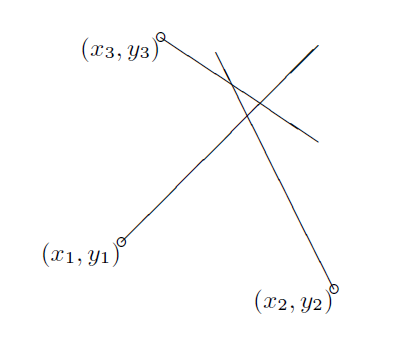
\includegraphics[width=6cm]{bearing.png}
\end{figure}

The sailor's rule of thumb says that the boat's position can be taken to be the centre of the cocked hat, the triangle produced by the intersection of the three measured bearings as in the figure shown. Can you persuade him that the maximum likelihood answer is better?
\begin{solution}
\end{solution}


% Bayesian Decision theory generalizations
\question[5] [{\sc Reverend Bayes decides}] 
\begin{parts}
\part[2] Consider a classification problem in which the loss incurred on mis-classifying an input vector from class $C_k$  as $C_j$ is given by loss matrix entry $L_{kj}$, and for which the loss incurred in selecting the reject option is $\psi$. Find the decision criterion that will give minimum expected loss, and then simplify it for the case of 0-1 loss (i.e., when $L_{kj} = 1 - I_{kj}$, with $I_{kj}$ being $1$ for $k=j$ and 0 otherwise).
\begin{solution}
\end{solution}

\part[2] 
Let $L$ be the loss matrix defined by $L=\begin{bmatrix}
 0 &1 &2\\
 1 &0 &1\\
 2 &1 &0
\end{bmatrix}$ where $L_{ij}$ indicates the loss for an input x with $i$ being the true class and $j$ the predicted class. All the three classes are equally likely to occur. The class densities are $P(x|C_1=1) \sim N(-2,1)$, $P(x|C_2=2) \sim N(0,1)$ and $P(x|C_3) \sim N(2,1)$. Find the Bayes classifier $h(x)$.
\begin{solution}
\end{solution}

\part[1]  Consider two classes $C_1$ and $C_2$ with equal priors and with class conditional densities of a feature $x$ given by Gaussian distributions with respective means $\mu_1$ and $\mu_2$, and same variance $\sigma^2$. Find equation of the decision boundary between these two classes.
\begin{solution}
\end{solution}
\end{parts}


\question[10][{\sc Don't mix your words!}]\newline
Consider two documents $D_1, D_2$ and a background language model given by a Categorical distribution (i.e., assume $P(w|\theta)$ is known for every word $w$ in the vocabulary $V$). We use the maximum likelihood method to estimate a unigram language model based on $D_1$, which will be denoted by $\theta_1$ (i.e, p(w|$\theta_1$) = ``nos. of times word w occurred in $D_1$''/|$D_1$|, where |$D_1$| denotes the total number of words in $D_1$). Assume document $D_2$ is generated by sampling words from a two-component Categorical mixture model where one component is $p(w|\theta_1)$ and the other is $p(w|\theta)$. Let $\lambda$ denote the probability that $D_1$ would be selected to generate a word in $D_2$. That makes $1-\lambda$ the probability of selecting the background model. Let $D_2 = (w_1,w_2, ....w_k)$, where $w_i$ is a word from the vocabulary $V$. Use the mixture model to fit $D_2$ and compute the ML estimate of $\lambda$ using the EM (Expectation-Maximization) algorithm.
\begin{parts}
\part[2] Given that each word $w_i$ in document $D_2$ is generated independently from the mixture model, write down the log-likelihood of the whole document $D_2$. Is it easy to maximize this log-likelihood? 
\begin{solution}
\end{solution}

\part[4] Write down the E-step and M-step updating formulas for estimating $\lambda$. Show your derivation of these formulas.
\begin{solution}
\end{solution}

\part[4] In the previous parts of the question, we assume that the background language model $P(w|\theta)$ is known. How will your E-step and M-step change if you do not know the parameter $\theta$ and only know $\theta_1$? Show your derivation. 
\begin{solution}
\end{solution}

\part[3] {\sc [Bonus]} The previous parts of the question deal with MLE based density estimation. If you were to employ a Bayesian estimation method to infer $\lambda$, how will you proceed? That is, what prior would you choose for $\lambda$, and what is the the formula for the posterior? Is this posterior easily computable (i.e., has a closed-form expression or can be computed efficiently)? You can assume that both $P(w|\theta_1)$ and $P(w|\theta)$ are known and only $\lambda$ is not known. 
\begin{solution}
\end{solution}
\end{parts}


\question[10] [{\sc Density estimation - the one ring to rule them all!}]
With density estimation ring already in your finger, you have all you need to master simple linear regression (even before seeing regression formally in class). Simple linear regression is a model that assumes a linear relationship between an input (aka independent) variable $x$ and an output (aka dependent) variable $y$.
\newline
Let us assume that the available set of observations, $\mathbb{D} = {\{x_i, y_i\}}_{i=1}^{n}$, are iid samples from the following model that captures the relationship between $y$ and $x$: 
\[y_i = w_0 + w_1 x_i + \epsilon_i; \qquad \epsilon_i \sim \mathcal{N}(0,\sigma^2) \]
In this model, note that $x_i$ is not a random variable, whereas $\epsilon_i$ and hence $y_i$ are random variables, with $\epsilon_i$ being modeled as a Gaussian noise that is independent of each other and doesn't depend on $x_i$. Value of $\sigma$ is assumed to be known for simplicity.\newline
We would like to learn the parameters $\theta=\{w_0, w_1\}$ of the model, i.e., we would like to use MLE to estimate the exact parameter values or Bayesian methods to infer the (posterior) probability distribution over the parameter values.

\begin{parts}
\part[2]
Compute the probability distribution $P(y_i | x_i,\theta)$, and use it to write down the log likelihood of the model. 
\begin{solution}
\end{solution}

\part[3] Derive the ML estimates for $w_0$ and $w_1$ by optimizing the above log likelihood. 
\begin{solution}
\end{solution}

\part[2] If $\sigma$ is also not known before, derive the ML estimate for  $\sigma$.
\begin{solution}
\end{solution}

\part[3] 
For Bayesian inference, assume that the parameters $w_0, w_1$ are independent of each other and follow the distributions $\mathcal{N}(\mu_0, \sigma_0^2)$ and $\mathcal{N}(\mu_1, \sigma_1^2)$ respectively. Compute the posterior distributions for each parameter. How does the mode of this posterior (i.e., MAP estimate) relate to the MLE of $w_0$ and $w_1$ derived above?
\begin{solution}
\end{solution}
\end{parts}


\question[10] [{\sc Let's roll up your coding sleeves...}]
\textbf{Learning Binary Bayes Classifiers from data via Density Estimation}\\
Derive Bayes classifiers under assumptions below and employing maximum likelihood approach to estimate class prior/conditional densities, and return the results on a test set.
\begin{enumerate}
\item \textbf{BayesA} Assume $X|Y=-1 \sim \mathcal{N}(\mu_-, I)$ and  $X|Y=1 \sim \mathcal{N}(\mu_+, I)$ 
\item \textbf{BayesB} Assume $X|Y=-1 \sim \mathcal{N}(\mu_-, \Sigma)$ and $X|Y=1 \sim \mathcal{N}(\mu_+, \Sigma)$ 
\item \textbf{BayesC} Assume $X|Y=-1 \sim \mathcal{N}(\mu_-, \Sigma_-)$ and $X|Y=1 \sim \mathcal{N}(\mu_+, \Sigma_+)$ 
\end{enumerate}
Please see \href{https://drive.google.com/drive/folders/1Ciew2xqnwD8V7D2PuRWzf8tpXLSVE7eQ?usp=sharing}{this folder} for the template .ipynb file containing the helper functions, and you've to add the missing code to this file (specifically, three functions function\_for\_A, function\_for\_B and function\_for\_C, and associated plotting/ROC code snippets) to implement the above three algorithms for the three datasets given in the same folder. 

Please provide your results/answers in the pdf file you upload to GradeScope, but please submit your code separately in \href{https://courses.iitm.ac.in/mod/assign/view.php?id=75983}{this} moodle link. The code submitted should be a rollno.zip file containing two files: rollno.ipynb file (including your code as well as the exact same results/plots uploaded to Gradescope) and the associated rollno.py file.

\begin{parts}
\part[3] Plot all the classifiers (3 classification algorithms on $3$ datasets $= 9$ plots) on a 2D plot, Add the training data points also on the plots. (Color the positively classified area light green, and negatively classified area light red as in Fig 4.5 in Bishop's book). 
\begin{solution}
\end{solution}

\part[3] Give the ROC curves for all the classifiers. Note that a ROC curve plots the FPR (False Positive Rate) on the x-axis and TPR (True Positive Rate) on the y-axis. (9 plots)
\begin{solution}
\end{solution}

\part[2] Provide the error rates for the above classifiers (three classifiers on the three datasets as $3\times3$ table, with appropriately named rows and columns).  
\begin{solution}
\end{solution}

\part[2] Summarise and explain your observations based on your plots and the assumptions given in the problem. Also briefly comment whether a non-parametric density estimation approach could have been used to solve this problem, and if so, what the associated pros/cons are compared to the parametric MLE based approach you have implemented.   
\begin{solution}
\end{solution}
\end{parts}

\end{questions}
\end{document}

